\chapter{Modellazione dei Casi d'Uso}
\section{Attori e Casi d'Uso}
\begin{table}[!hbp]
	\centering
	\begin{tblr}{colspec=XX}
		\begin{minipage}[t]{\linewidth}
			\paragraph{Attori primari}
			\begin{itemize}[leftmargin=*]
				\item UtenteNonRegistrato
				\item UtenteRegistrato
				\item Utente
				\item Amministratore
			\end{itemize}
		\end{minipage} &
		\begin{minipage}[t]{\linewidth}
			\paragraph{Attori secondari}
			\begin{itemize}[leftmargin=*]
				\item SistemaGestioneAcquisti
			\end{itemize}
		\end{minipage} \\
	\end{tblr}
\end{table}
\begin{table}[!hbp]
	\centering
	\begin{tblr}{colspec=XX}
		\begin{minipage}[t]{\linewidth}
			\paragraph{Casi d'uso}
			\begin{enumerate}[leftmargin=*]
				\item Registrazione 
				\item Autenticazione
				\item RicercaEvento
				\item PubblicaEvento
				\item ConsultaEventiPubblicati
				\item PartecipazioneEvento
				\item AcquistoBiglietto
				\item ModificaDatiPersonali
				\item VisualizzaBiglietto
				\item ScaricaBiglietto
			\end{enumerate}
		\end{minipage} &
		\begin{minipage}[t]{\linewidth}
			\paragraph{Casi d'uso di inclusione}
			\begin{enumerate}[leftmargin=*, start=11]
                \item ConsultaCatalogoEventi
	      		\item ConsultaStoricoBiglietti
			\end{enumerate}

		\end{minipage}
	\end{tblr}
\end{table}
\begin{table}[!ht]
\centering
\small
\begin{tblr}{
  colspec = {X[2,l] X[1.2,l] X[1.7,l] X[1.6,l] X[1.5,l]},
  hlines,
  row{1} = {font=\bfseries}
}
Caso d'uso & Attori Primari & Attori Secondari & Incl. / Ext. & Requisiti corrispondenti \\
Registrazione & UtenteNonRegistrato & -- & -- & \Req{rf}{01} \\
Autenticazione & UtenteRegistrato & -- & -- & \Req{rf}{02} \\
RicercaEvento & UtenteRegistrato & -- & -- &\Req{rf}{08} \\
PubblicaEvento & Amministratore & -- & -- & \Req{rf}{06} \\
ConsultaEventiPubblicati & Amministratore & -- & Include: Consulta Catalogo Eventi & \Req{rf}{13}, \Req{rf}{14} \\
PartecipazioneEvento& Utente & -- & -- & \Req{rf}{12} \\
AcquistaBiglietto & Utente & SistemaGestioneAcquisti & Include: ConsultaCatalogoEventi & \Req{rf}{09} \\
ModificaDatiPersonali & Utente & -- & -- & \Req{rf}{05} \\
VisualizzaBiglietto & Utente & -- & -- & \Req{rf}{10} \\
ScaricaBiglietto & Utente & -- & -- & \Req{rf}{11} \\
ConsultaStoricoBiglietti & Utente & -- & --  & \Req{rf}{04} \\
ConsultaCatalogoEventi & UtenteRegistrato & --  & -- & \Req{rf}{07} \\

\end{tblr}
\end{table}

\section{Diagramma dei Casi d'Uso}
\begin{center}
\centering
	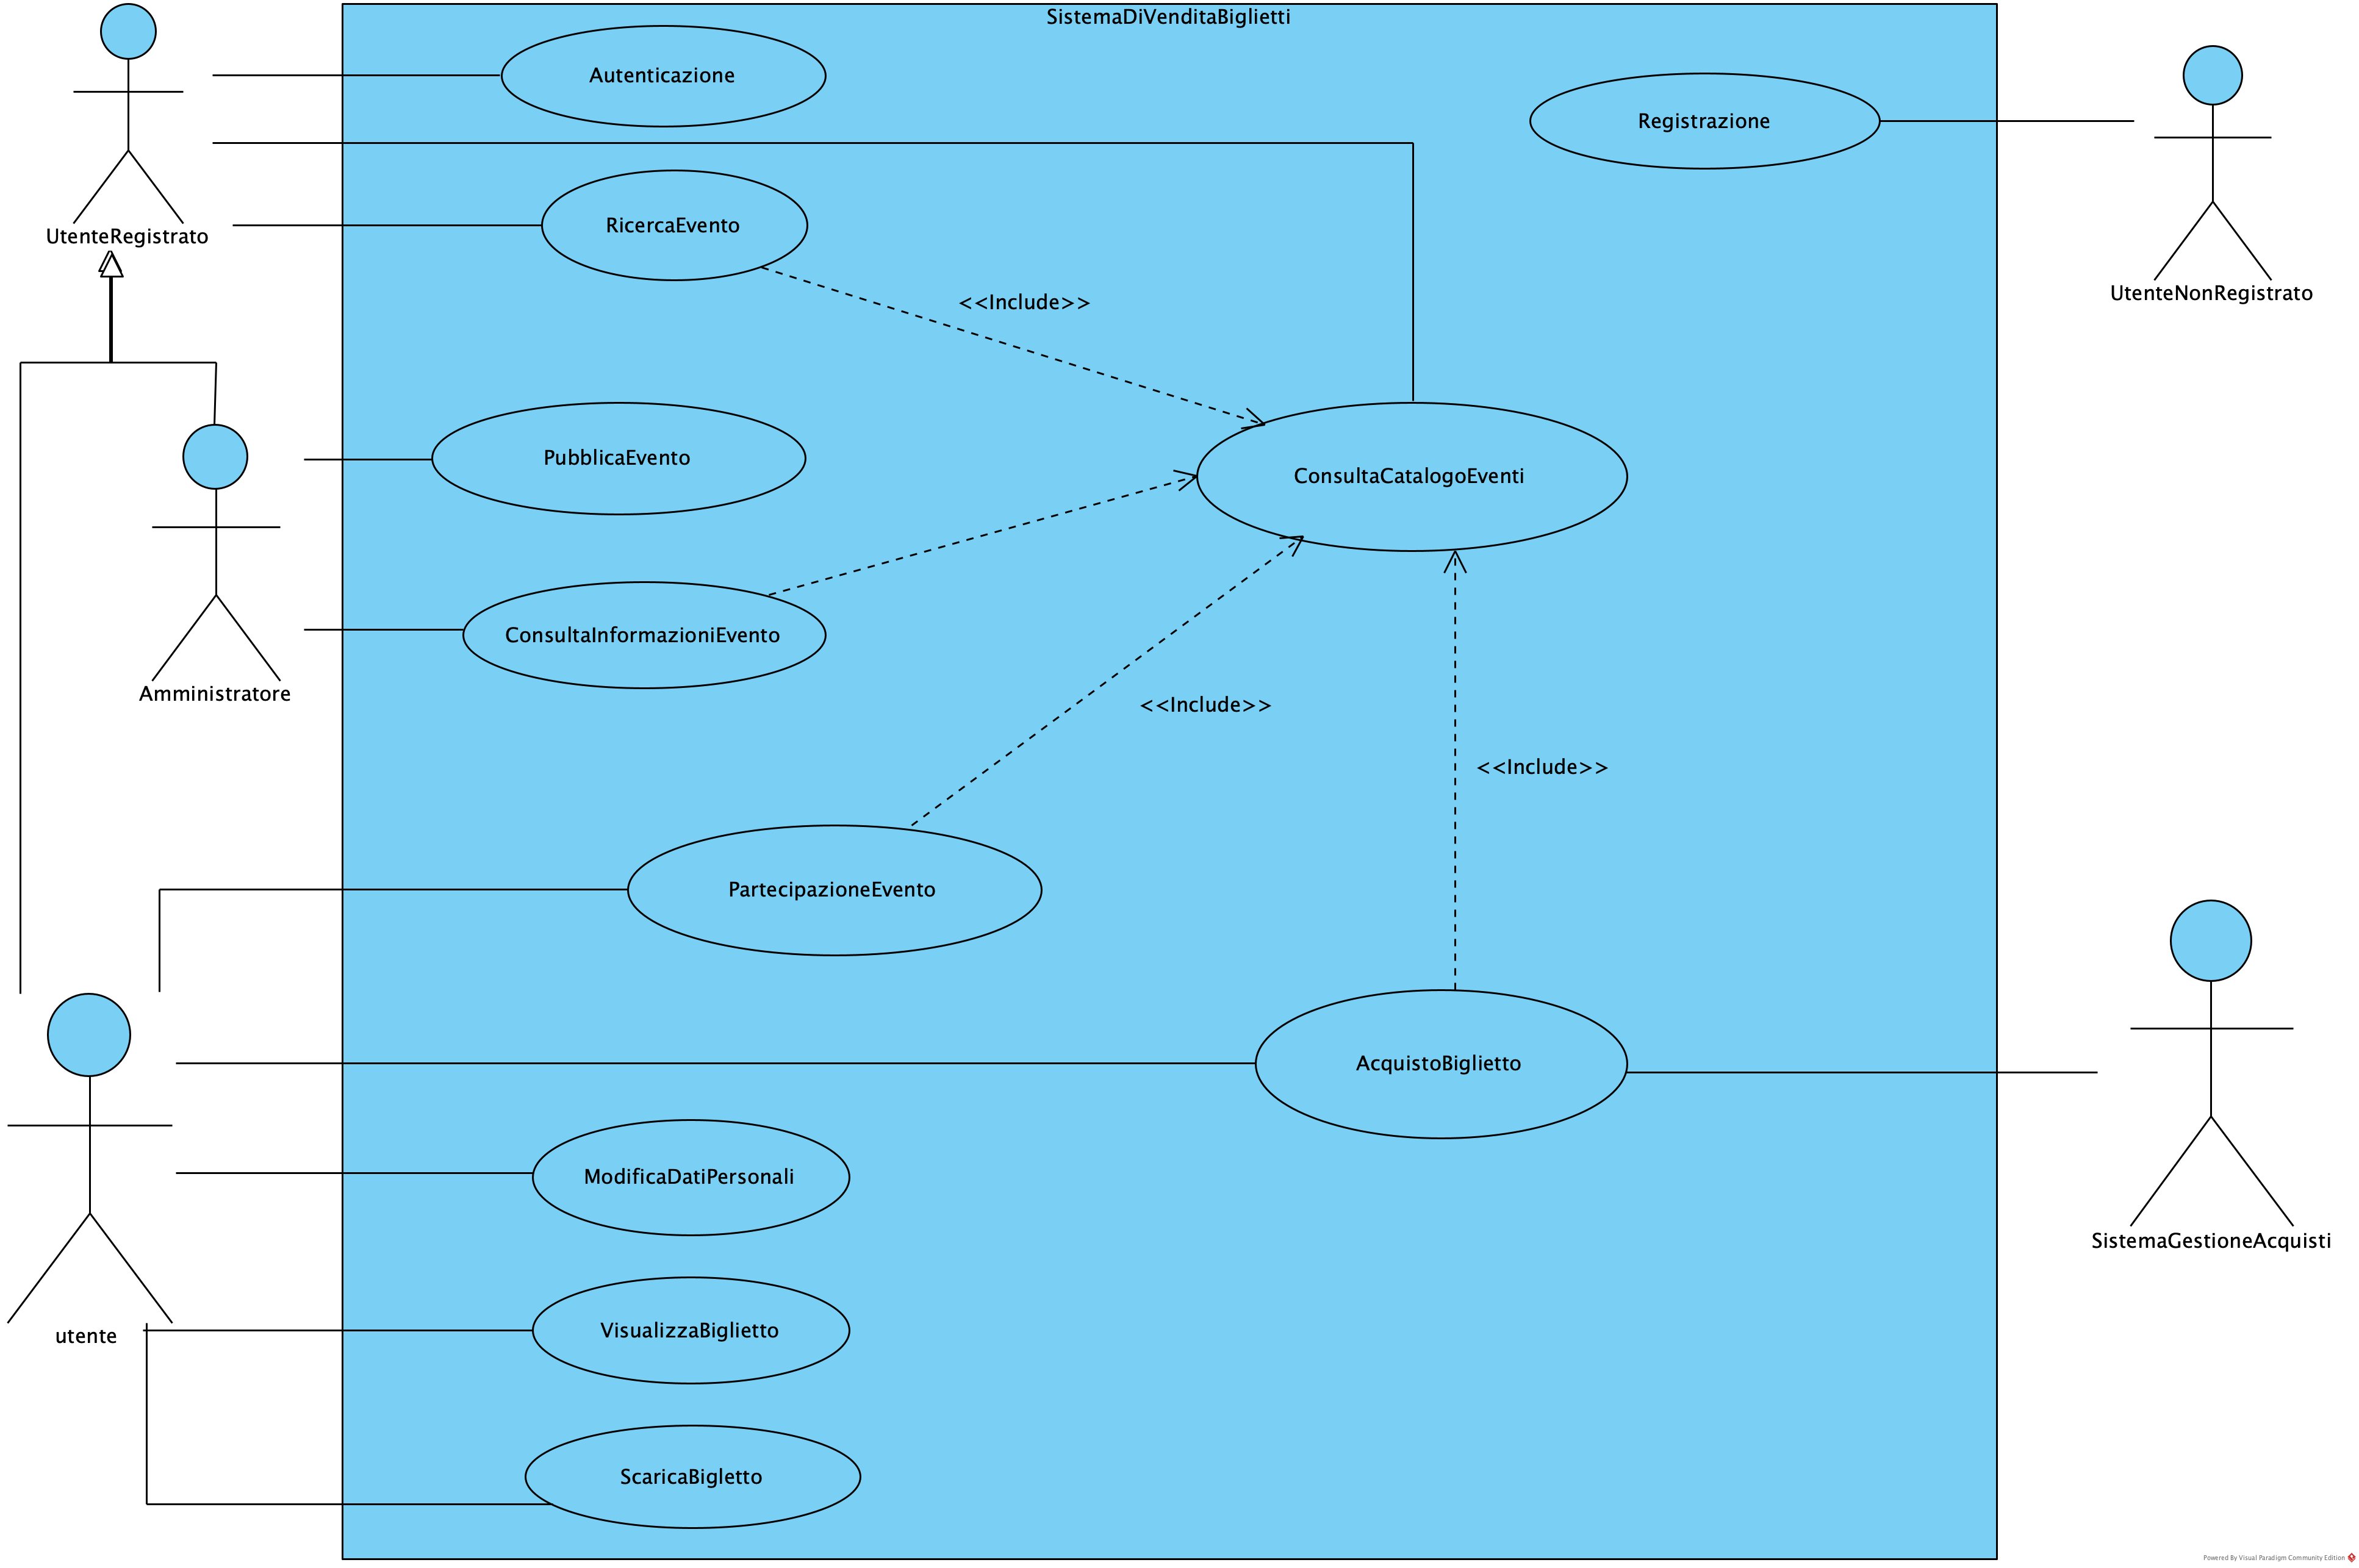
\includegraphics[width=\linewidth]{assets/casid'uso/usd.png}
\end{center}	

\clearpage
\section{Scenari}
\IncludeTable{capitoli/scenari/Registrazione}
\IncludeTable{capitoli/scenari/Autenticazione}
\IncludeTable{capitoli/scenari/RichiediCatalogoEventi}
\IncludeTable{capitoli/scenari/PartecipazioneEvento}
\IncludeTable{capitoli/scenari/PubblicaEvento}
\IncludeTable{capitoli/scenari/ConsultaEventiPubblicati}
\IncludeTable{capitoli/scenari/AcquistaBiglietto}

\newpage

\section{Diagramma delle Classi}

\begin{figure}[H]
	\centering
	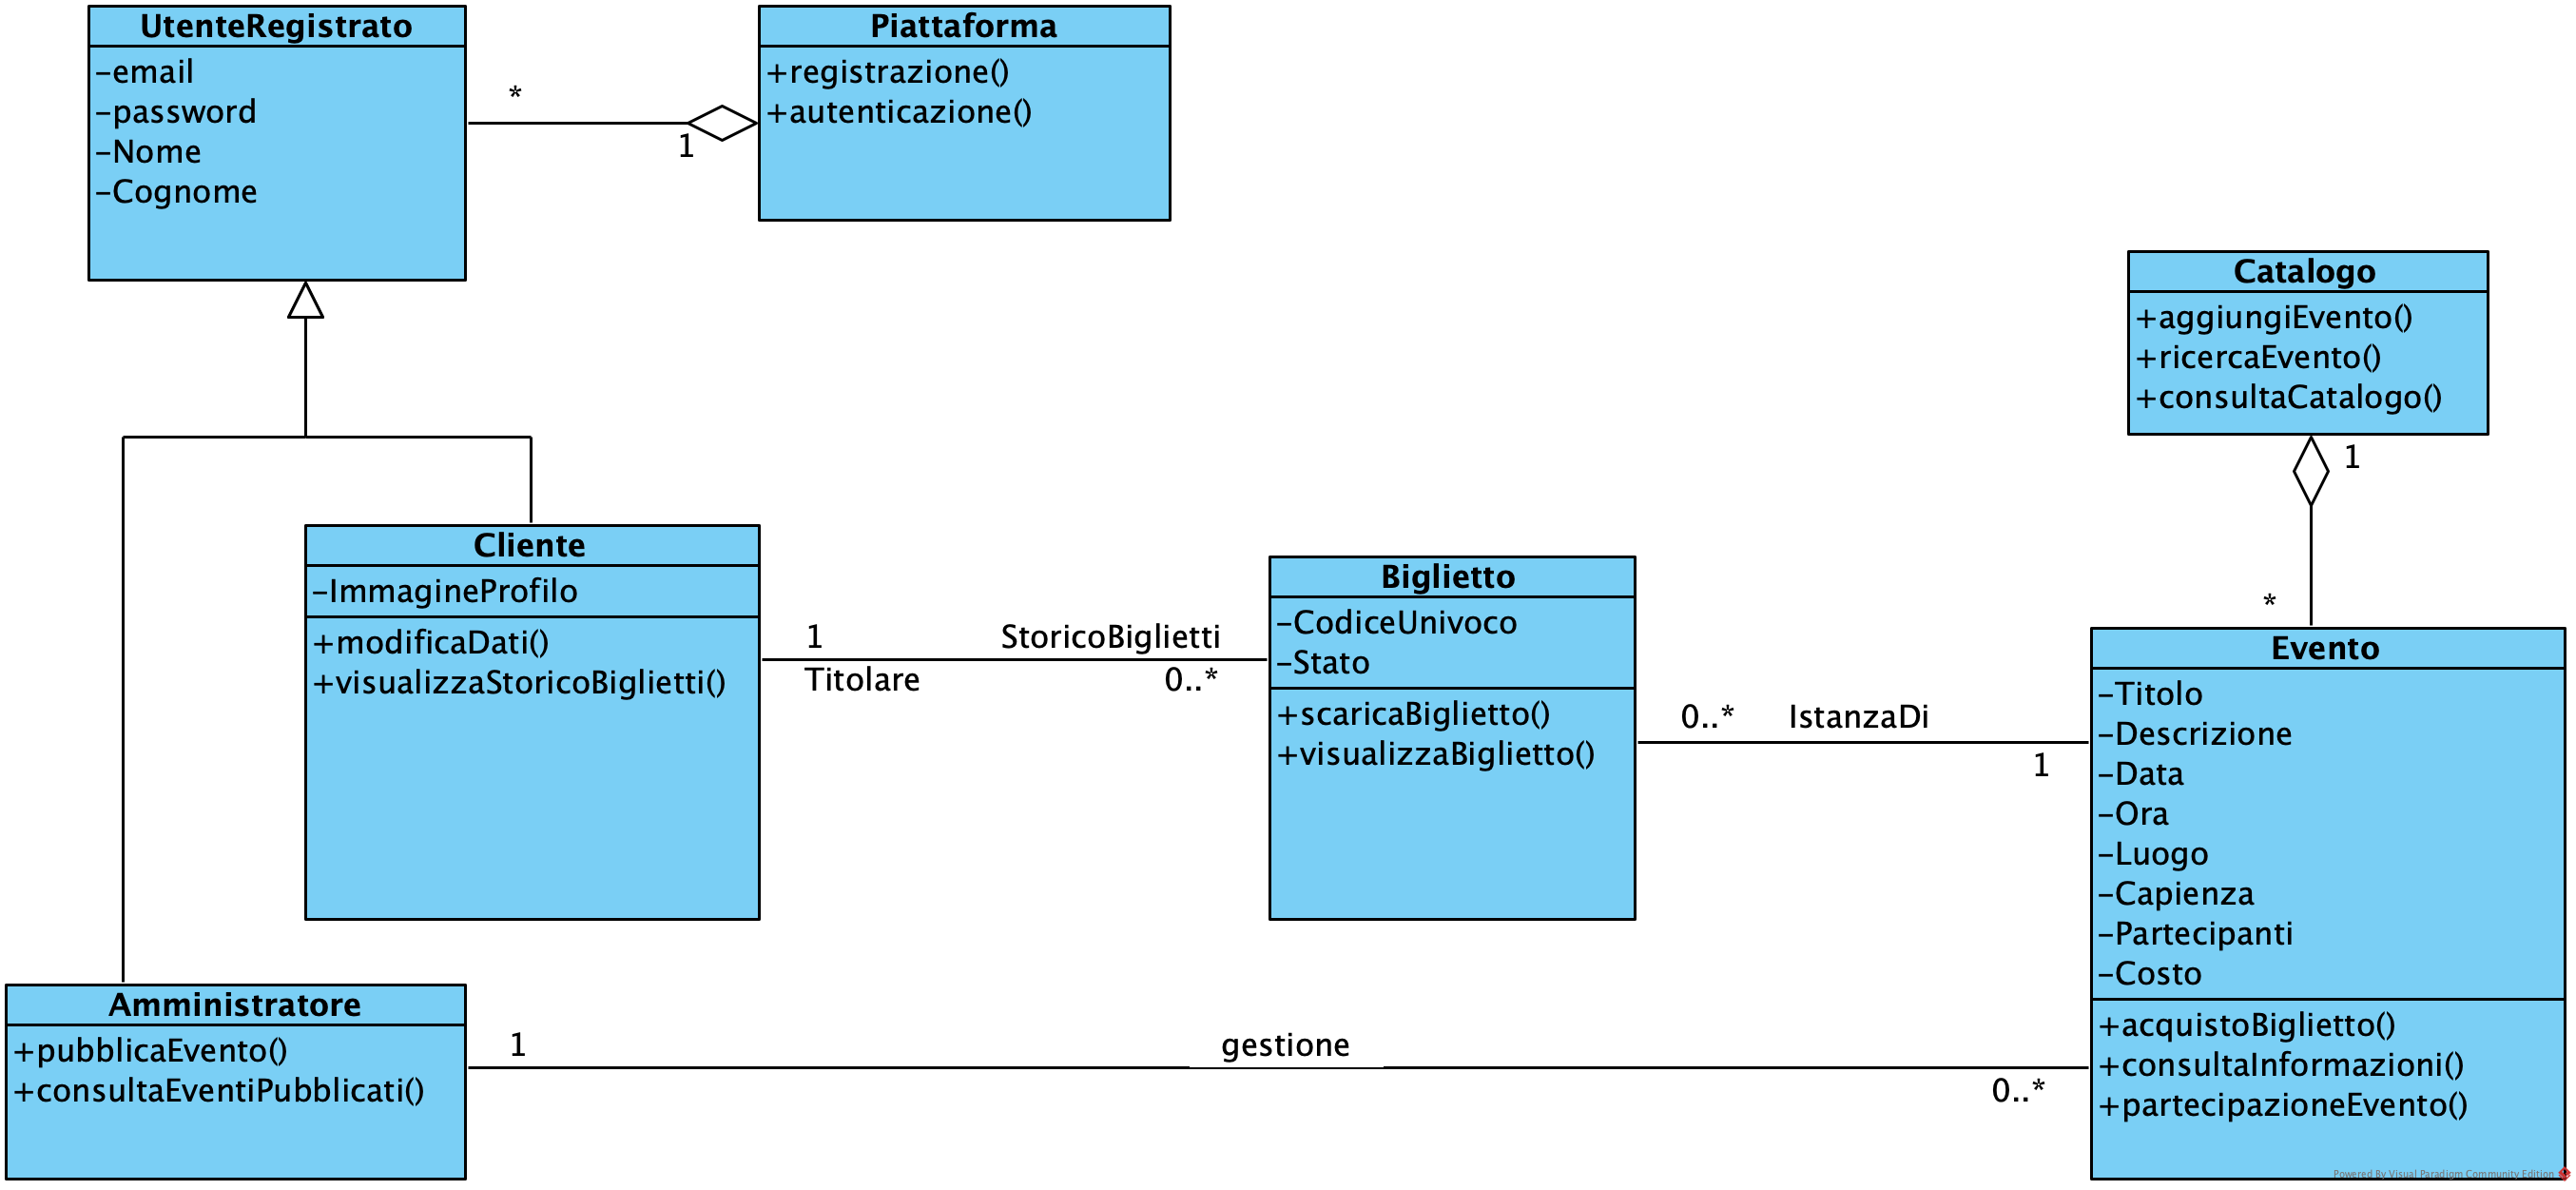
\includegraphics[width=0.8\linewidth]{assets/casid'uso/DiagrammaDelleClassi.png}
	\caption{Diagramma delle classi di analisi}
\end{figure}

\begin{table}[H]
	\centering
	\small % Riduce la dimensione del font
	\begin{tblr}{
	  colspec = {X[0.6,c] X[0.6,c]},
	  width = 1\linewidth, 
	  hlines, vlines,
	  row{1} = {bg=gray!30, font=\bfseries}
	}
	RESPONSABILITÀ & CLASSE \\
	Registrazione & Piattaforma \\
	Autenticazione & Piattaforma \\
	ModificaDati & Cliente \\
	VisualizzaStoricoBiglietti & Cliente \\
	CreazioneEvento & Amministratore \\
	ConsultaEventiPubblicati & Amministratore\\
	ScaricaBiglietto & Biglietto \\
	VisualizzaBiglietto & Biglietto \\
	AcquistoBiglietto & Evento \\
	PartecipazioneEvento & Evento \\
	ConsultaInformazioni & Evento \\
	AggiungiEvento & Catalogo \\
	RicercaEvento & Catalogo \\
	ConsultaCatalogo & Catalogo \\
	\end{tblr}
\end{table}

\vspace{-0.5em} % Riduce spazio tra tabella e testo
\begin{itemize}\setlength\itemsep{0.4em} % Riduce spazio tra gli item
    \item \textbf{Registrazione e Autenticazione:} \\
    Responsabilità della \textbf{Piattaforma}, in quanto \emph{Information Expert} di \texttt{UtenteRegistrato}.
    
    \item \textbf{ModificaDati e VisualizzaStoricoBiglietti:} \\
    Responsabilità del \textbf{Cliente}, poiché operano direttamente sui suoi attributi e sulle entità a lui associate.
    
    \item \textbf{AcquistoBiglietto:} \\
    Assegnata alla classe \textbf{Evento}, in quanto \emph{Creator} di un \texttt{Biglietto}.
    
    \item \textbf{PartecipazioneEvento:} \\
    Gestita dalla classe \textbf{Evento}, seguendo il principio di \emph{Low Coupling} per minimizzare le dipendenze tra classi.
    
    \item \textbf{RicercaEvento, AggiungiEvento e ConsultaCatalogo:} \\
    Responsabilità della classe \textbf{Catalogo}, in quanto \emph{Information Expert} degli \texttt{Eventi} presenti nel sistema.
    
    \item \textbf{CreazioneEvento:} \\
    Di competenza dell'\textbf{Amministratore}, in quanto \emph{Creator} di un \texttt{Evento}.
    
    \item \textbf{ConsultaEventiPubblicati:} \\
    Assegnata all'\textbf{Amministratore}, poiché \emph{Information Expert} degli eventi da lui gestiti e pubblicati.
\end{itemize}


\section{Diagrammi di sequenza}
\subsection{Registrazione}

La creazione del seguente diagramma di sequenza, ha fatto emergere la necessità di definire un metodo per la classe \textbf{Piattaforma}: \texttt{controlloEmail(Email)}, tale metodo consente alla \textbf{Piattaforma} di verificare che l'indirizzo email non sia già registrato nel sistema
\begin{figure}[H]
    \centering
    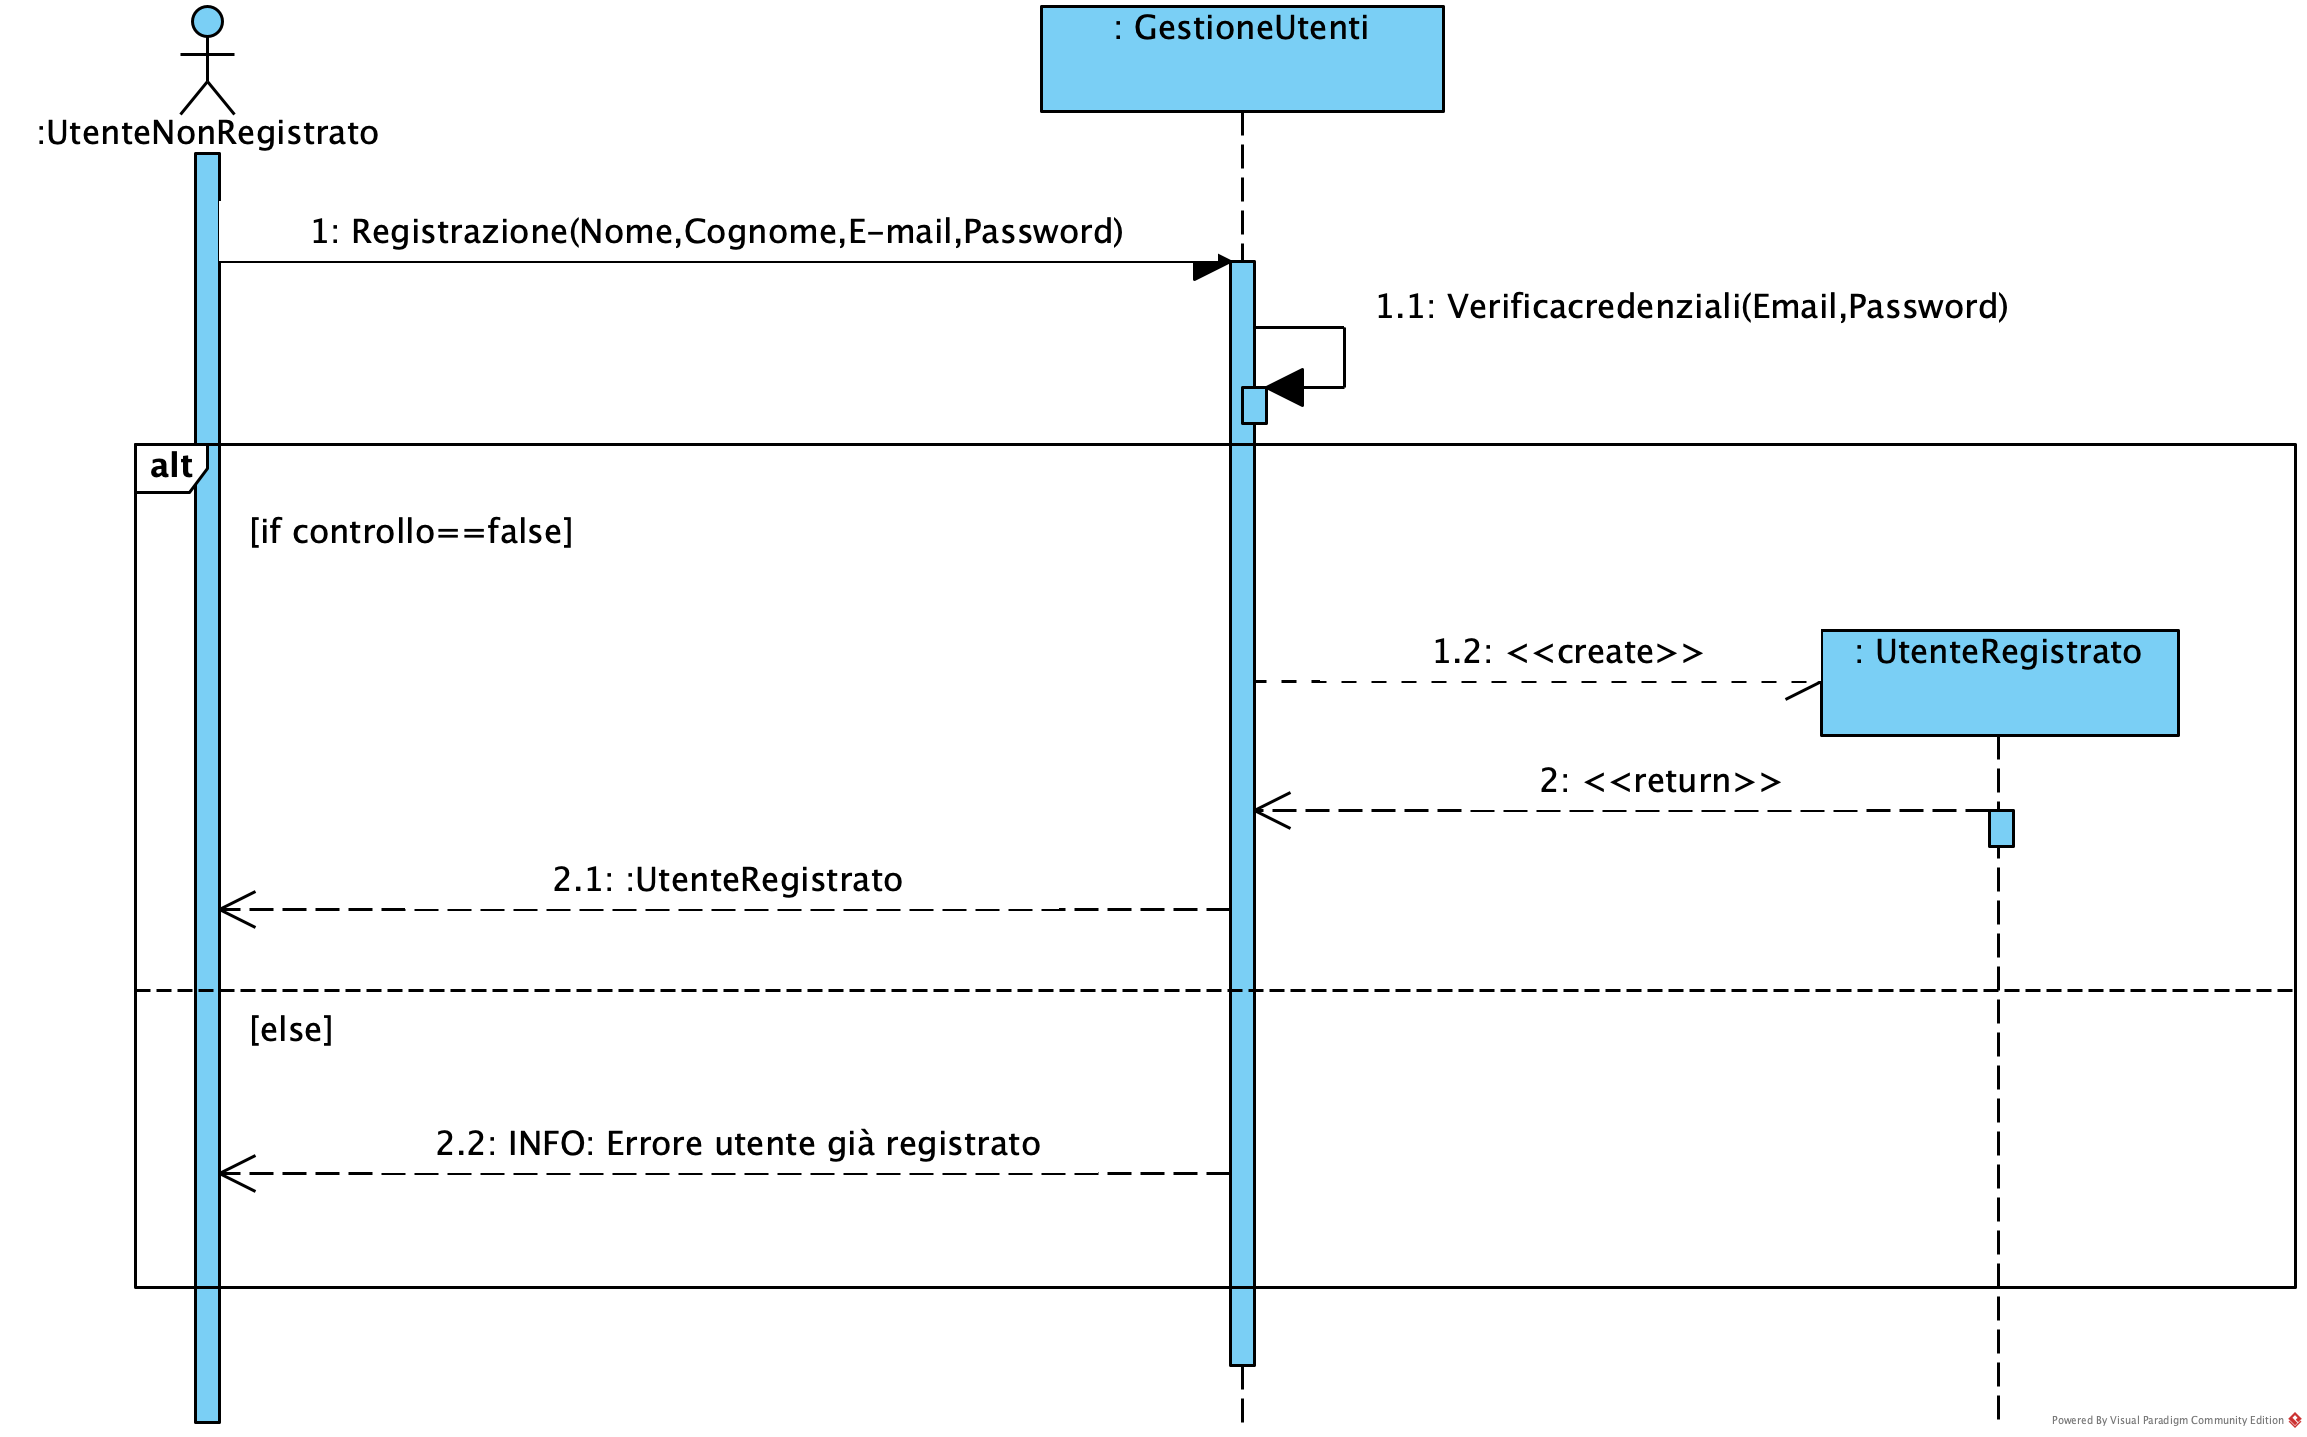
\includegraphics[width=0.8\linewidth]{assets/casid'uso/Registrazione.png}
    \caption{Diagramma di sequenza per il caso d'uso \emph{Registrazione}}
    \label{fig:registrazione}
\end{figure}

\subsection{Autenticazione}
Il diagramma di sequenza ha evidenziato la necessità del metodo \texttt{verificaCredenziali(password)} per la classe \textbf{UtenteRegistrato}, che permette di verificare la password inserita corrisponde a quella dell'utenteRegistrato.
\begin{figure}[H]
    \hspace{4cm}
    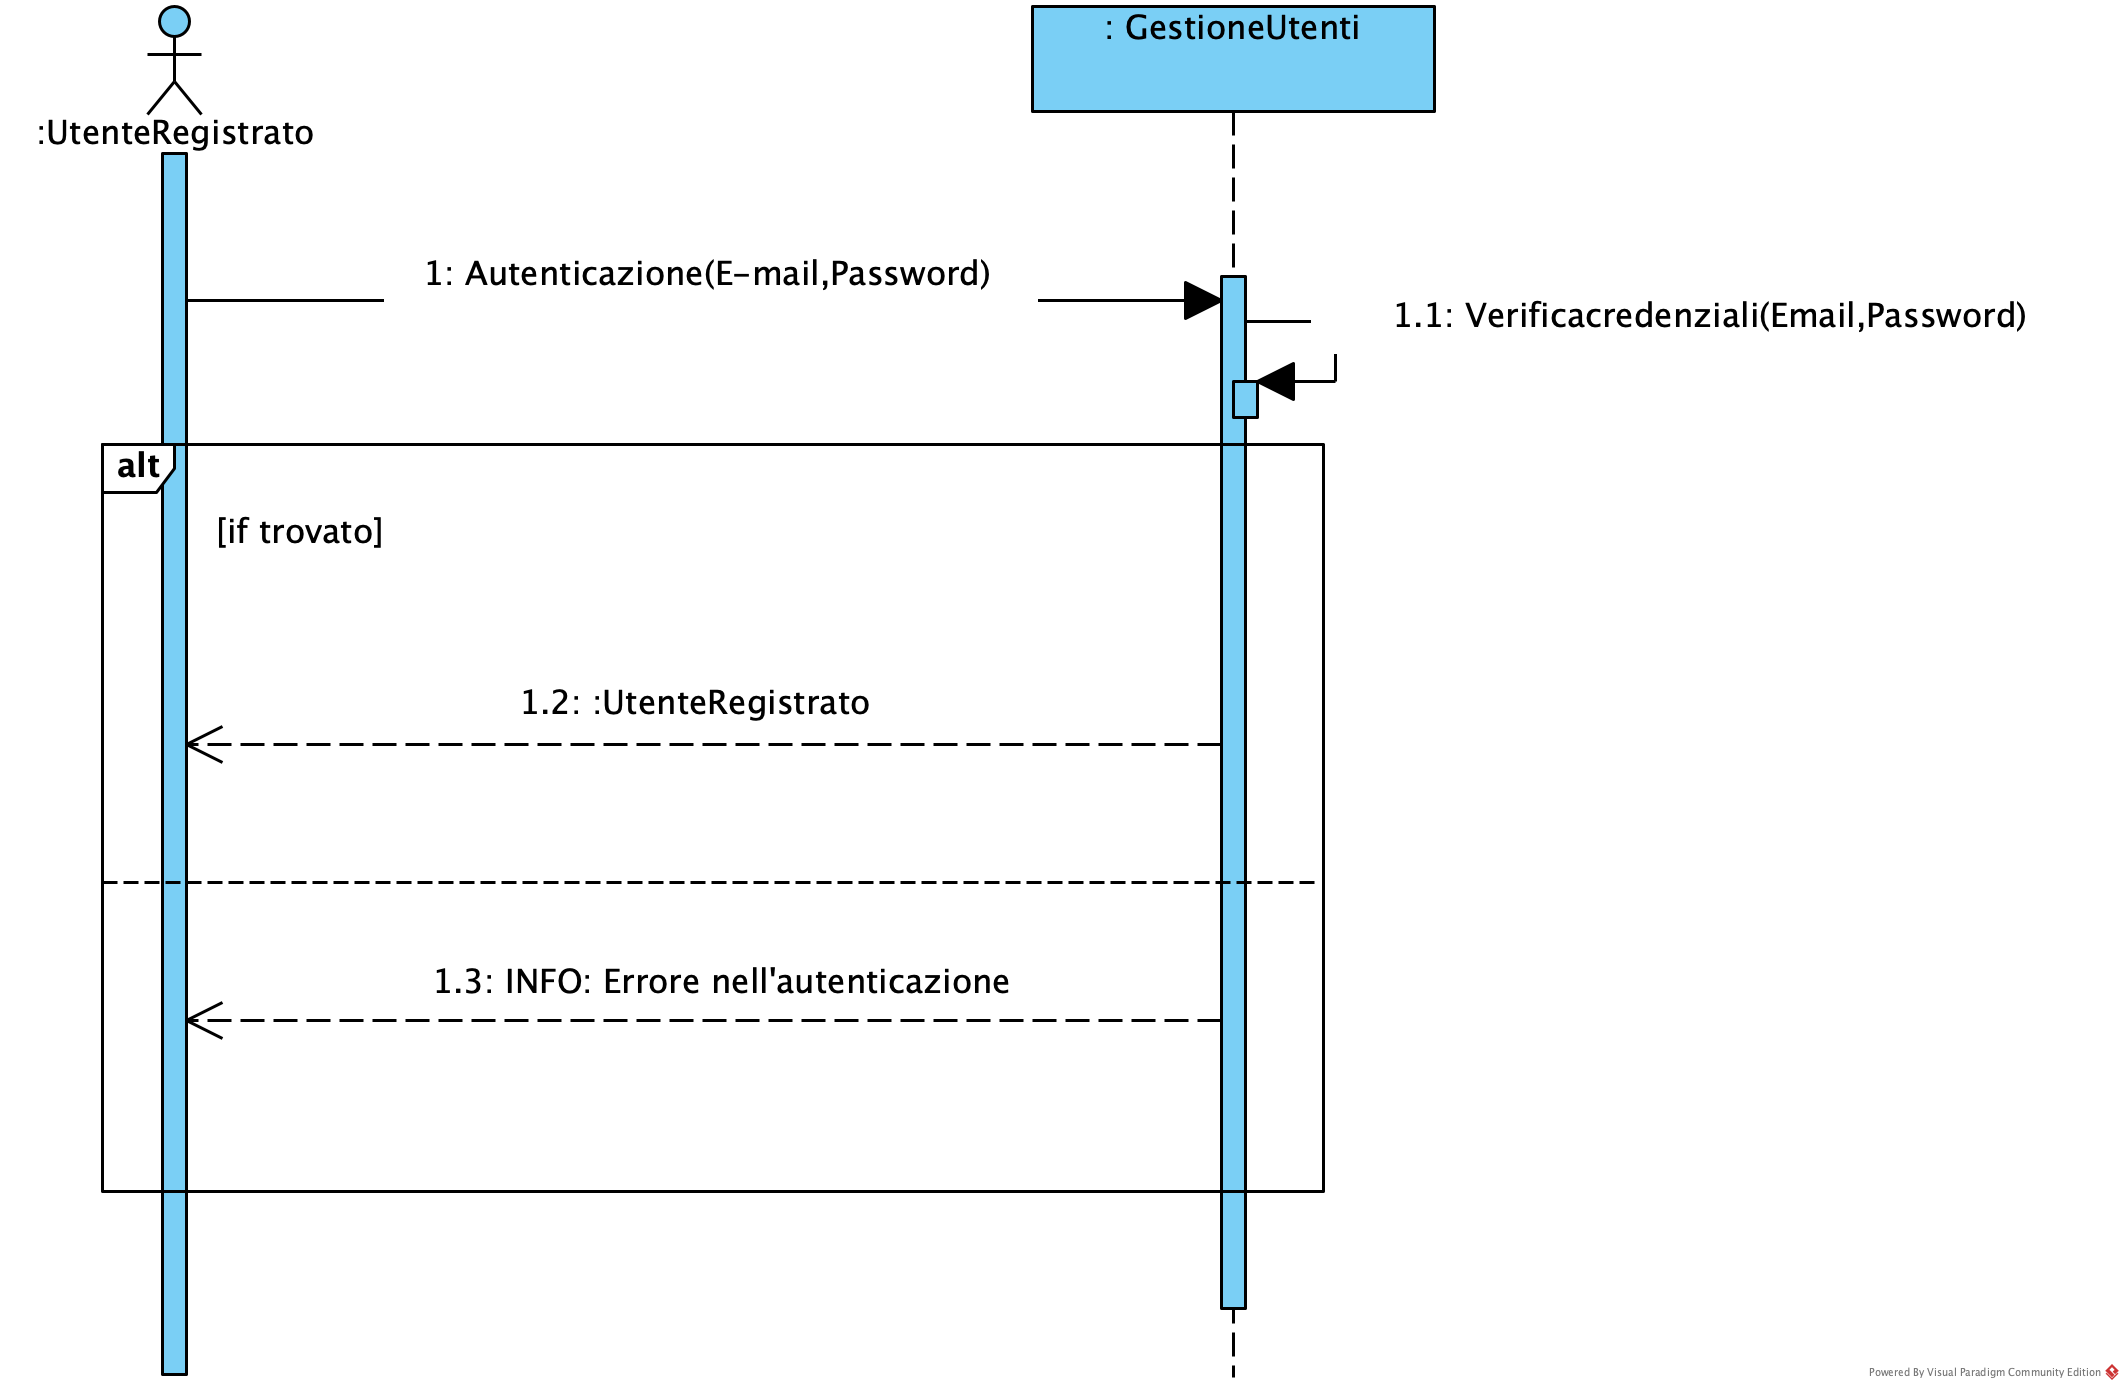
\includegraphics[width=0.8\linewidth]{assets/casid'uso/Autenticazione.png}
    \caption{Diagramma di sequenza per il caso d'uso \emph{Autenticazione}}
    \label{fig:autenticazione}
\end{figure}

\subsection{PubblicaEvento}

Il diagramma di sequenza ha evidenziato la necessità del metodo \texttt{verificaValidità(Titolo)} per la classe \textbf{Catalogo}, che permette di verificare che non esiste nel sistema un evento con lo stesso titolo.
Viene inoltre inserito un nuovo metodo \texttt{aggiungiEvento(Evento)} per la classe \texttt{Catalogo}, che permette di aggiungere al catalogo un nuovo evento.

\begin{figure}[H]
    \centering
    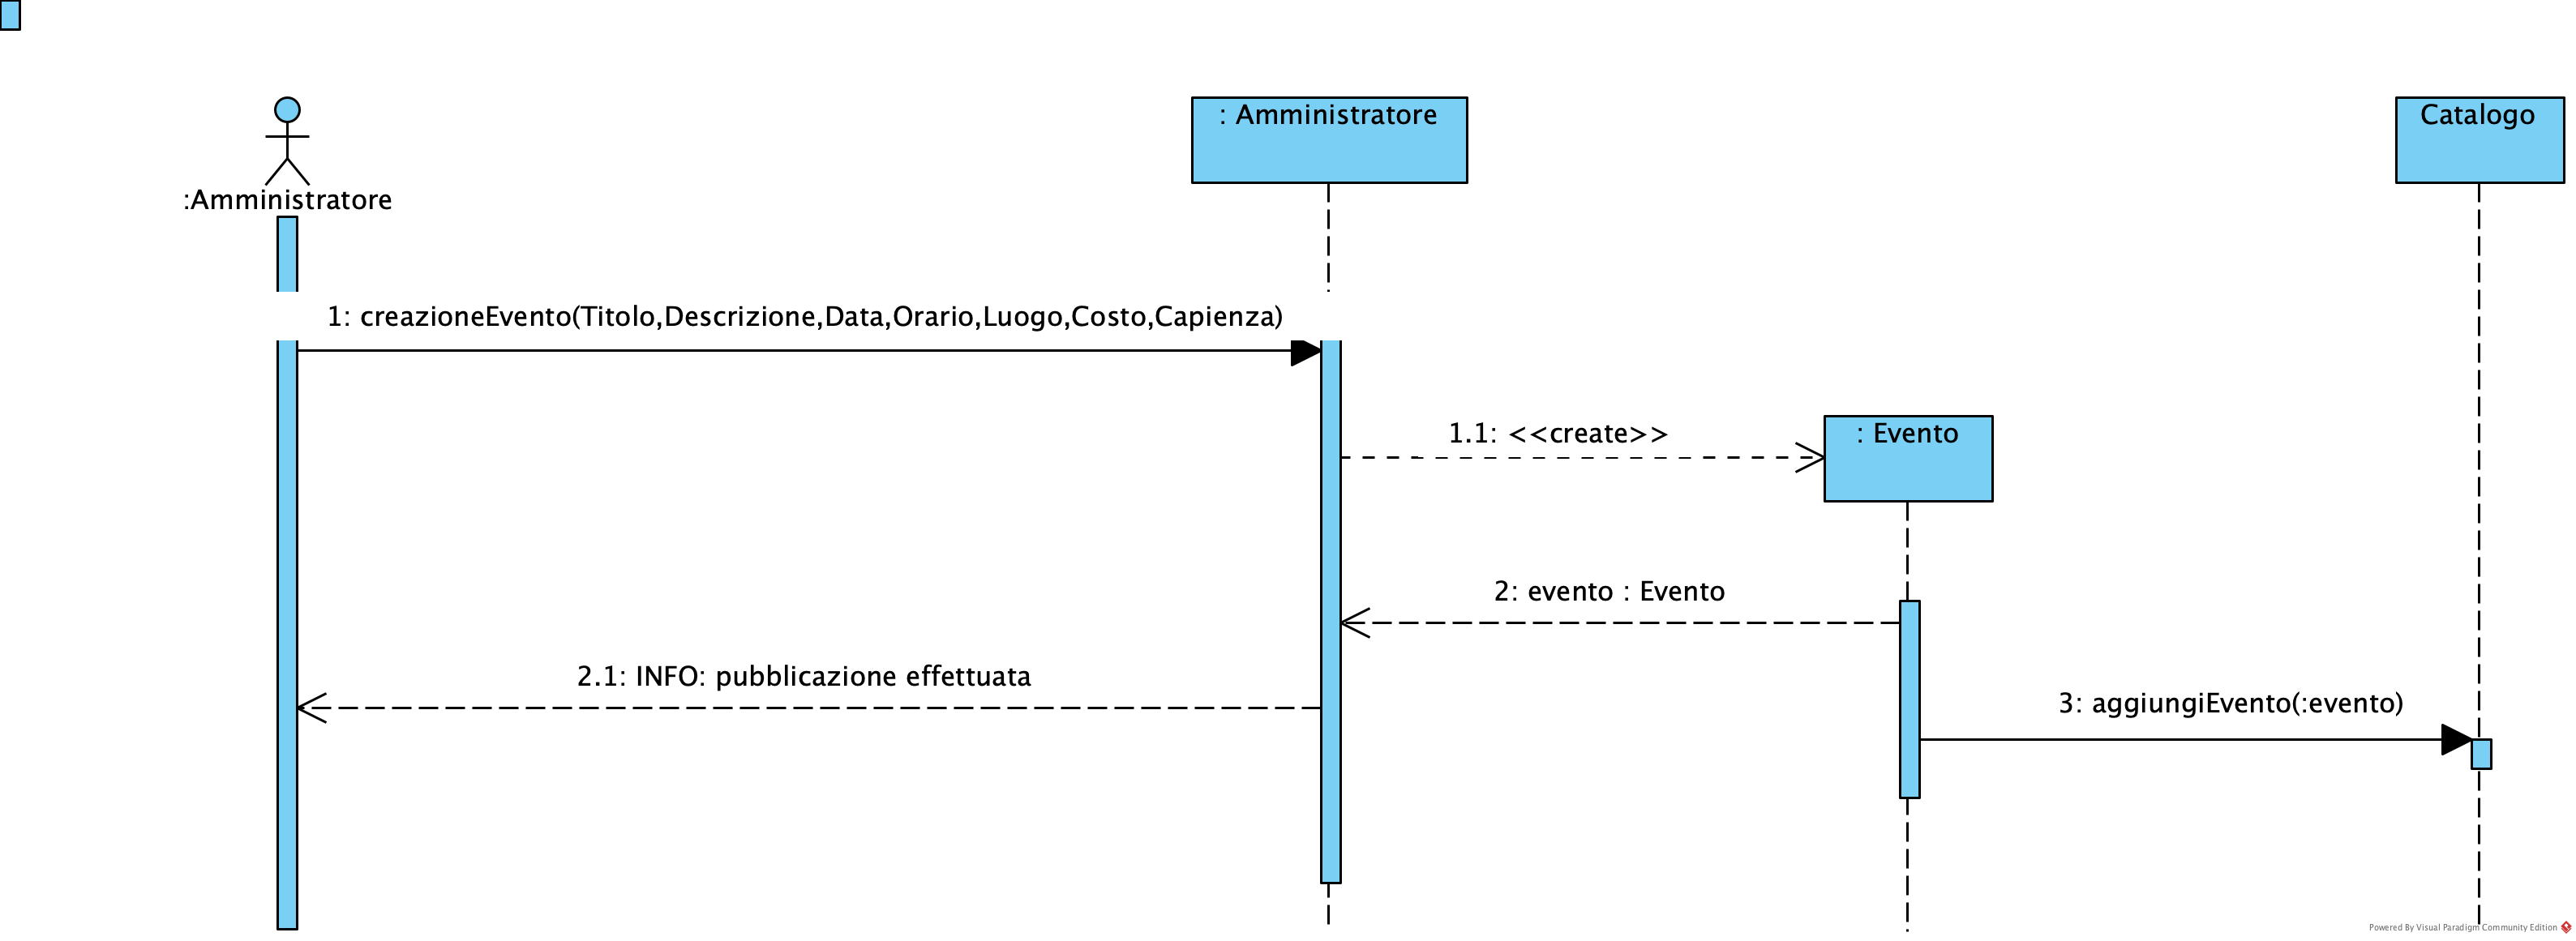
\includegraphics[width=\linewidth]{assets/casid'uso/PubblicaEvento.png}
    \caption{Diagramma di sequenza per il caso d'uso \emph{PubblicaEvento}}
    \label{fig:pubblicaevento}
\end{figure}

\subsection{ConsultaEventiPubblicati}

\begin{center}
    Il diagramma di sequenza del caso d'uso \textit{ConsultaEventiPubblicati} mostra la necessità di una responsabilità \textbf{getListaPartecipanti()} da parte dell'evento
    \vspace{2ex}
    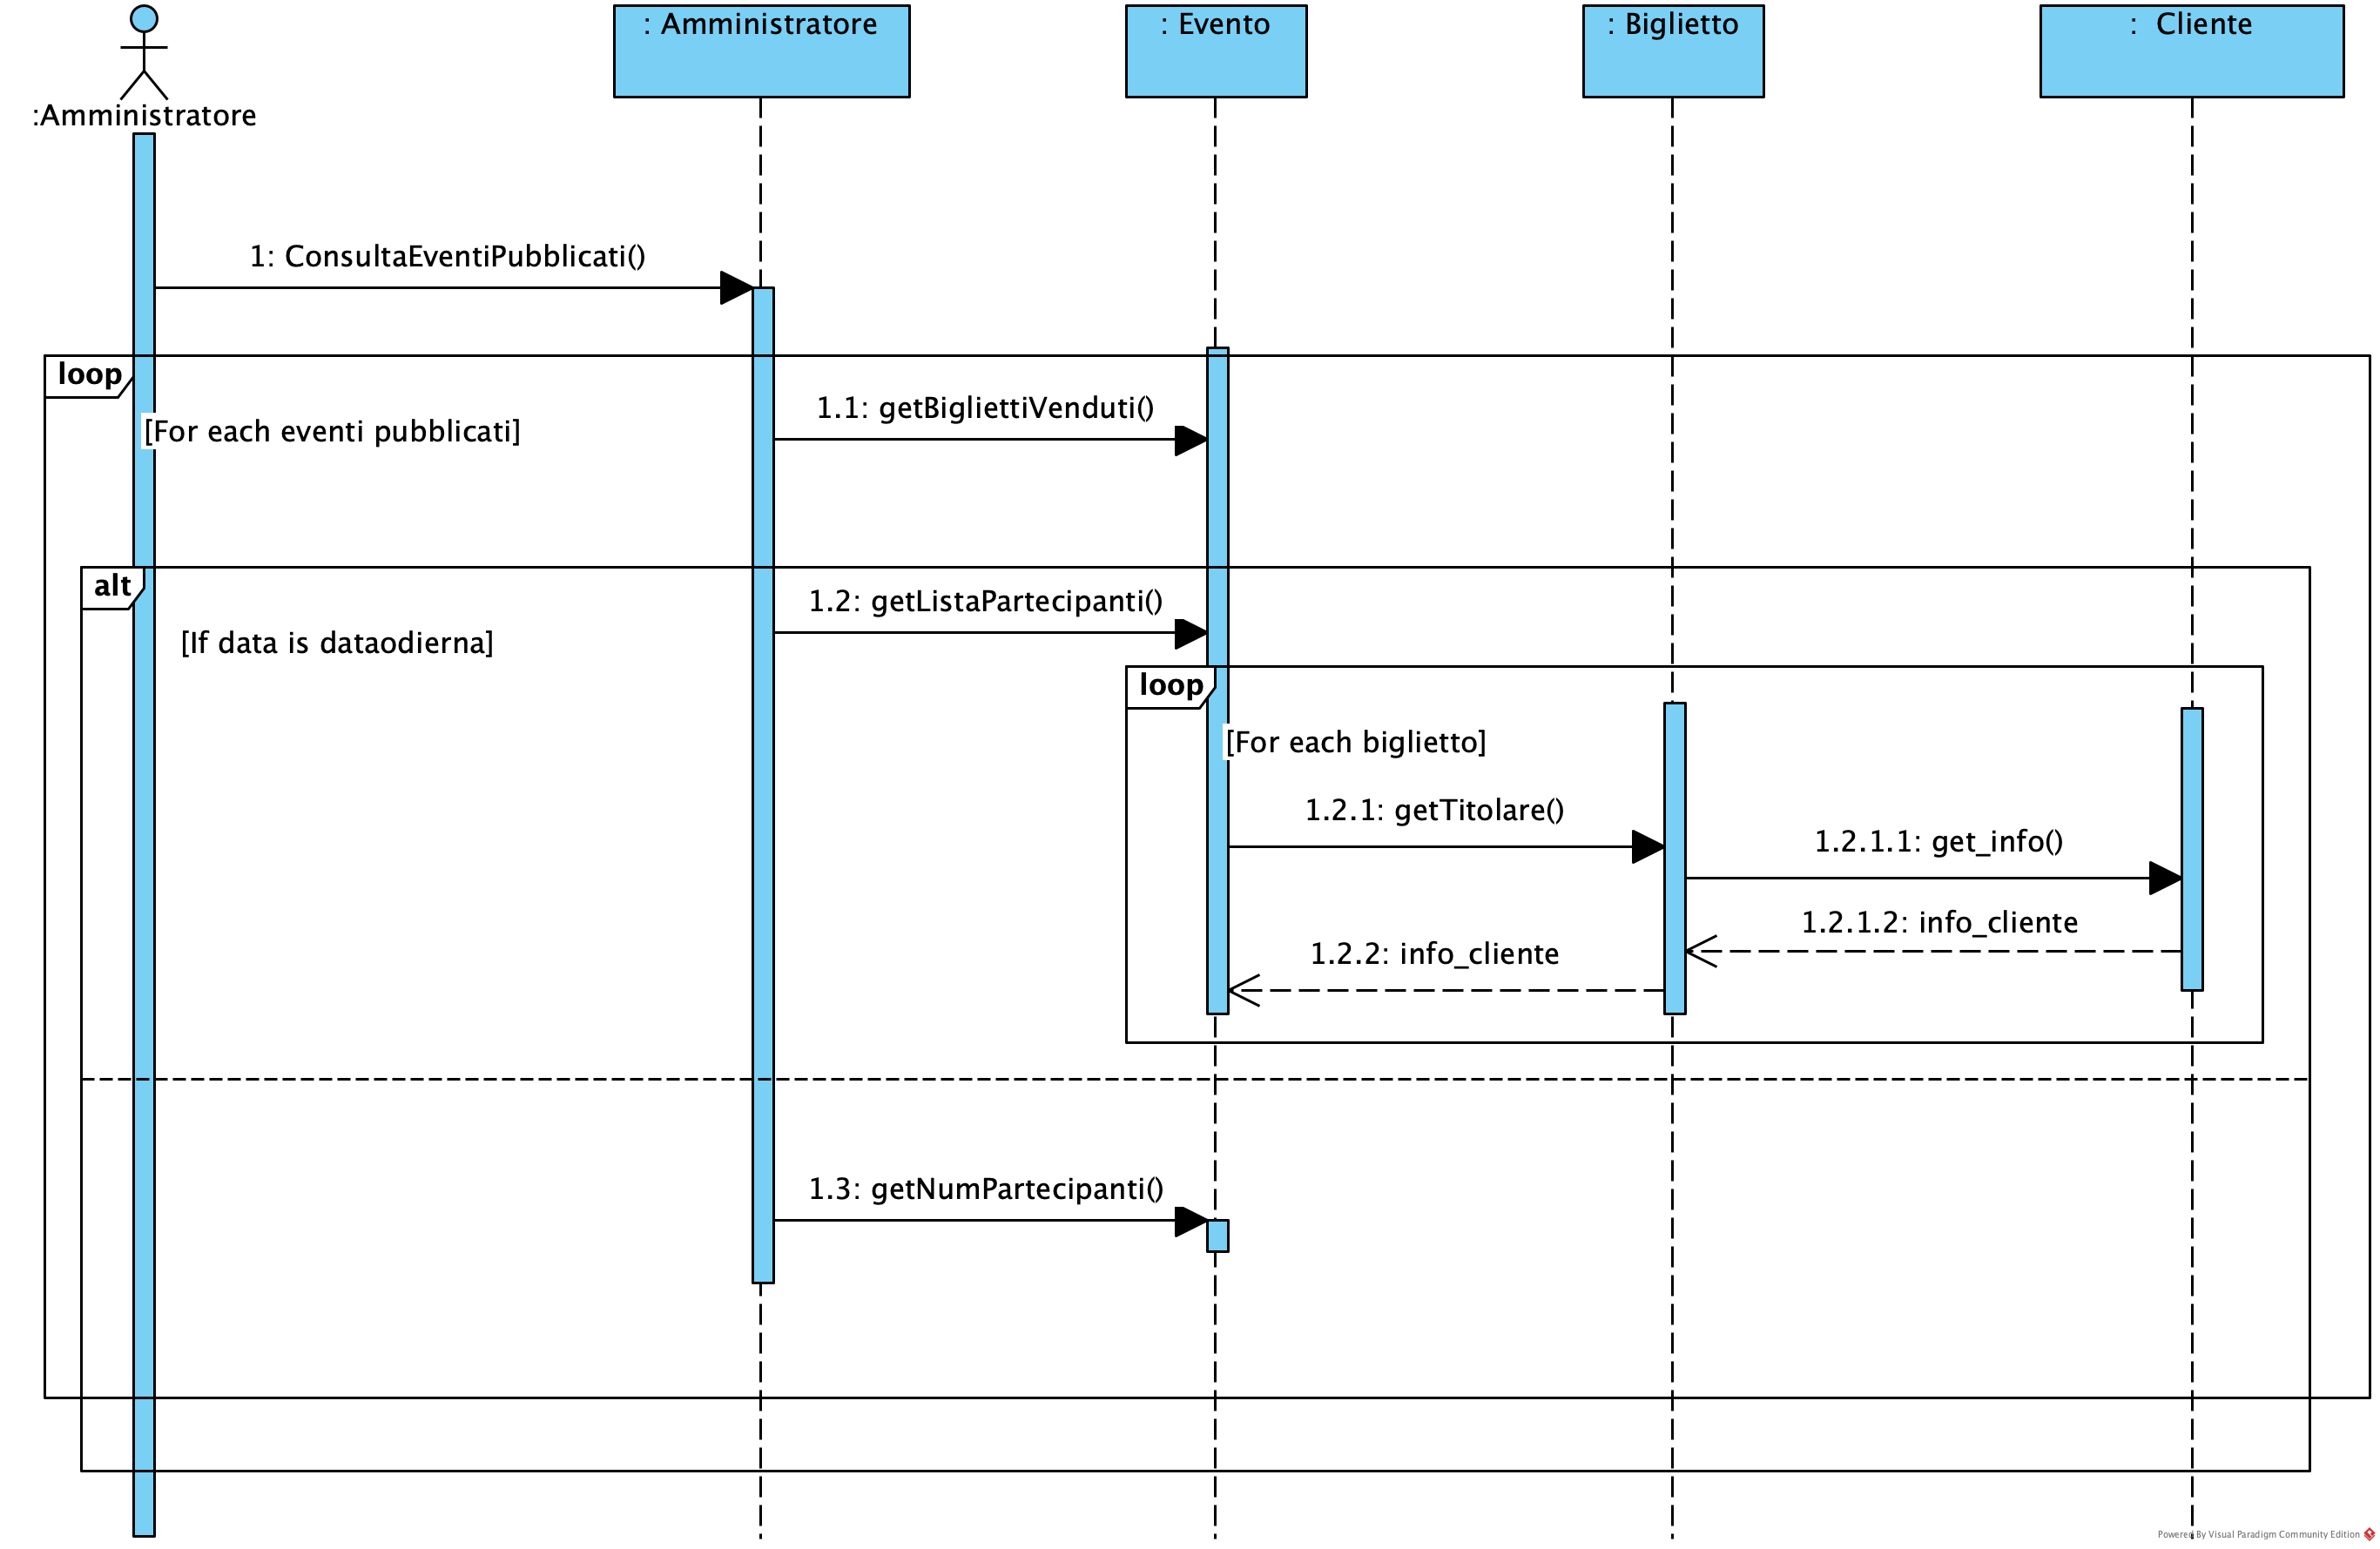
\includegraphics[width=0.8\linewidth]{assets/casid'uso/ConsultaEventiPubblicati.png}

    \vspace{1ex}
    \textbf{Figura:} Diagramma di sequenza per il caso d’uso \textit{ConsultaEventiPubblicati}
\end{center}

\newpage
\subsection{AcquistoBiglietti}

Il diagramma di sequenza ha evidenziato diverse responsabilità: per la classe \textbf{Evento} i metodi \texttt{verificaDisponibilità()}, \texttt{creazioneIdUnivoco()}, mentre per la classe \textbf{Cliente} il metodo \texttt{haBigliettoPerEvento(Evento)} per verificare eventuali acquisti precedenti.

\begin{figure}[H]
    \centering
    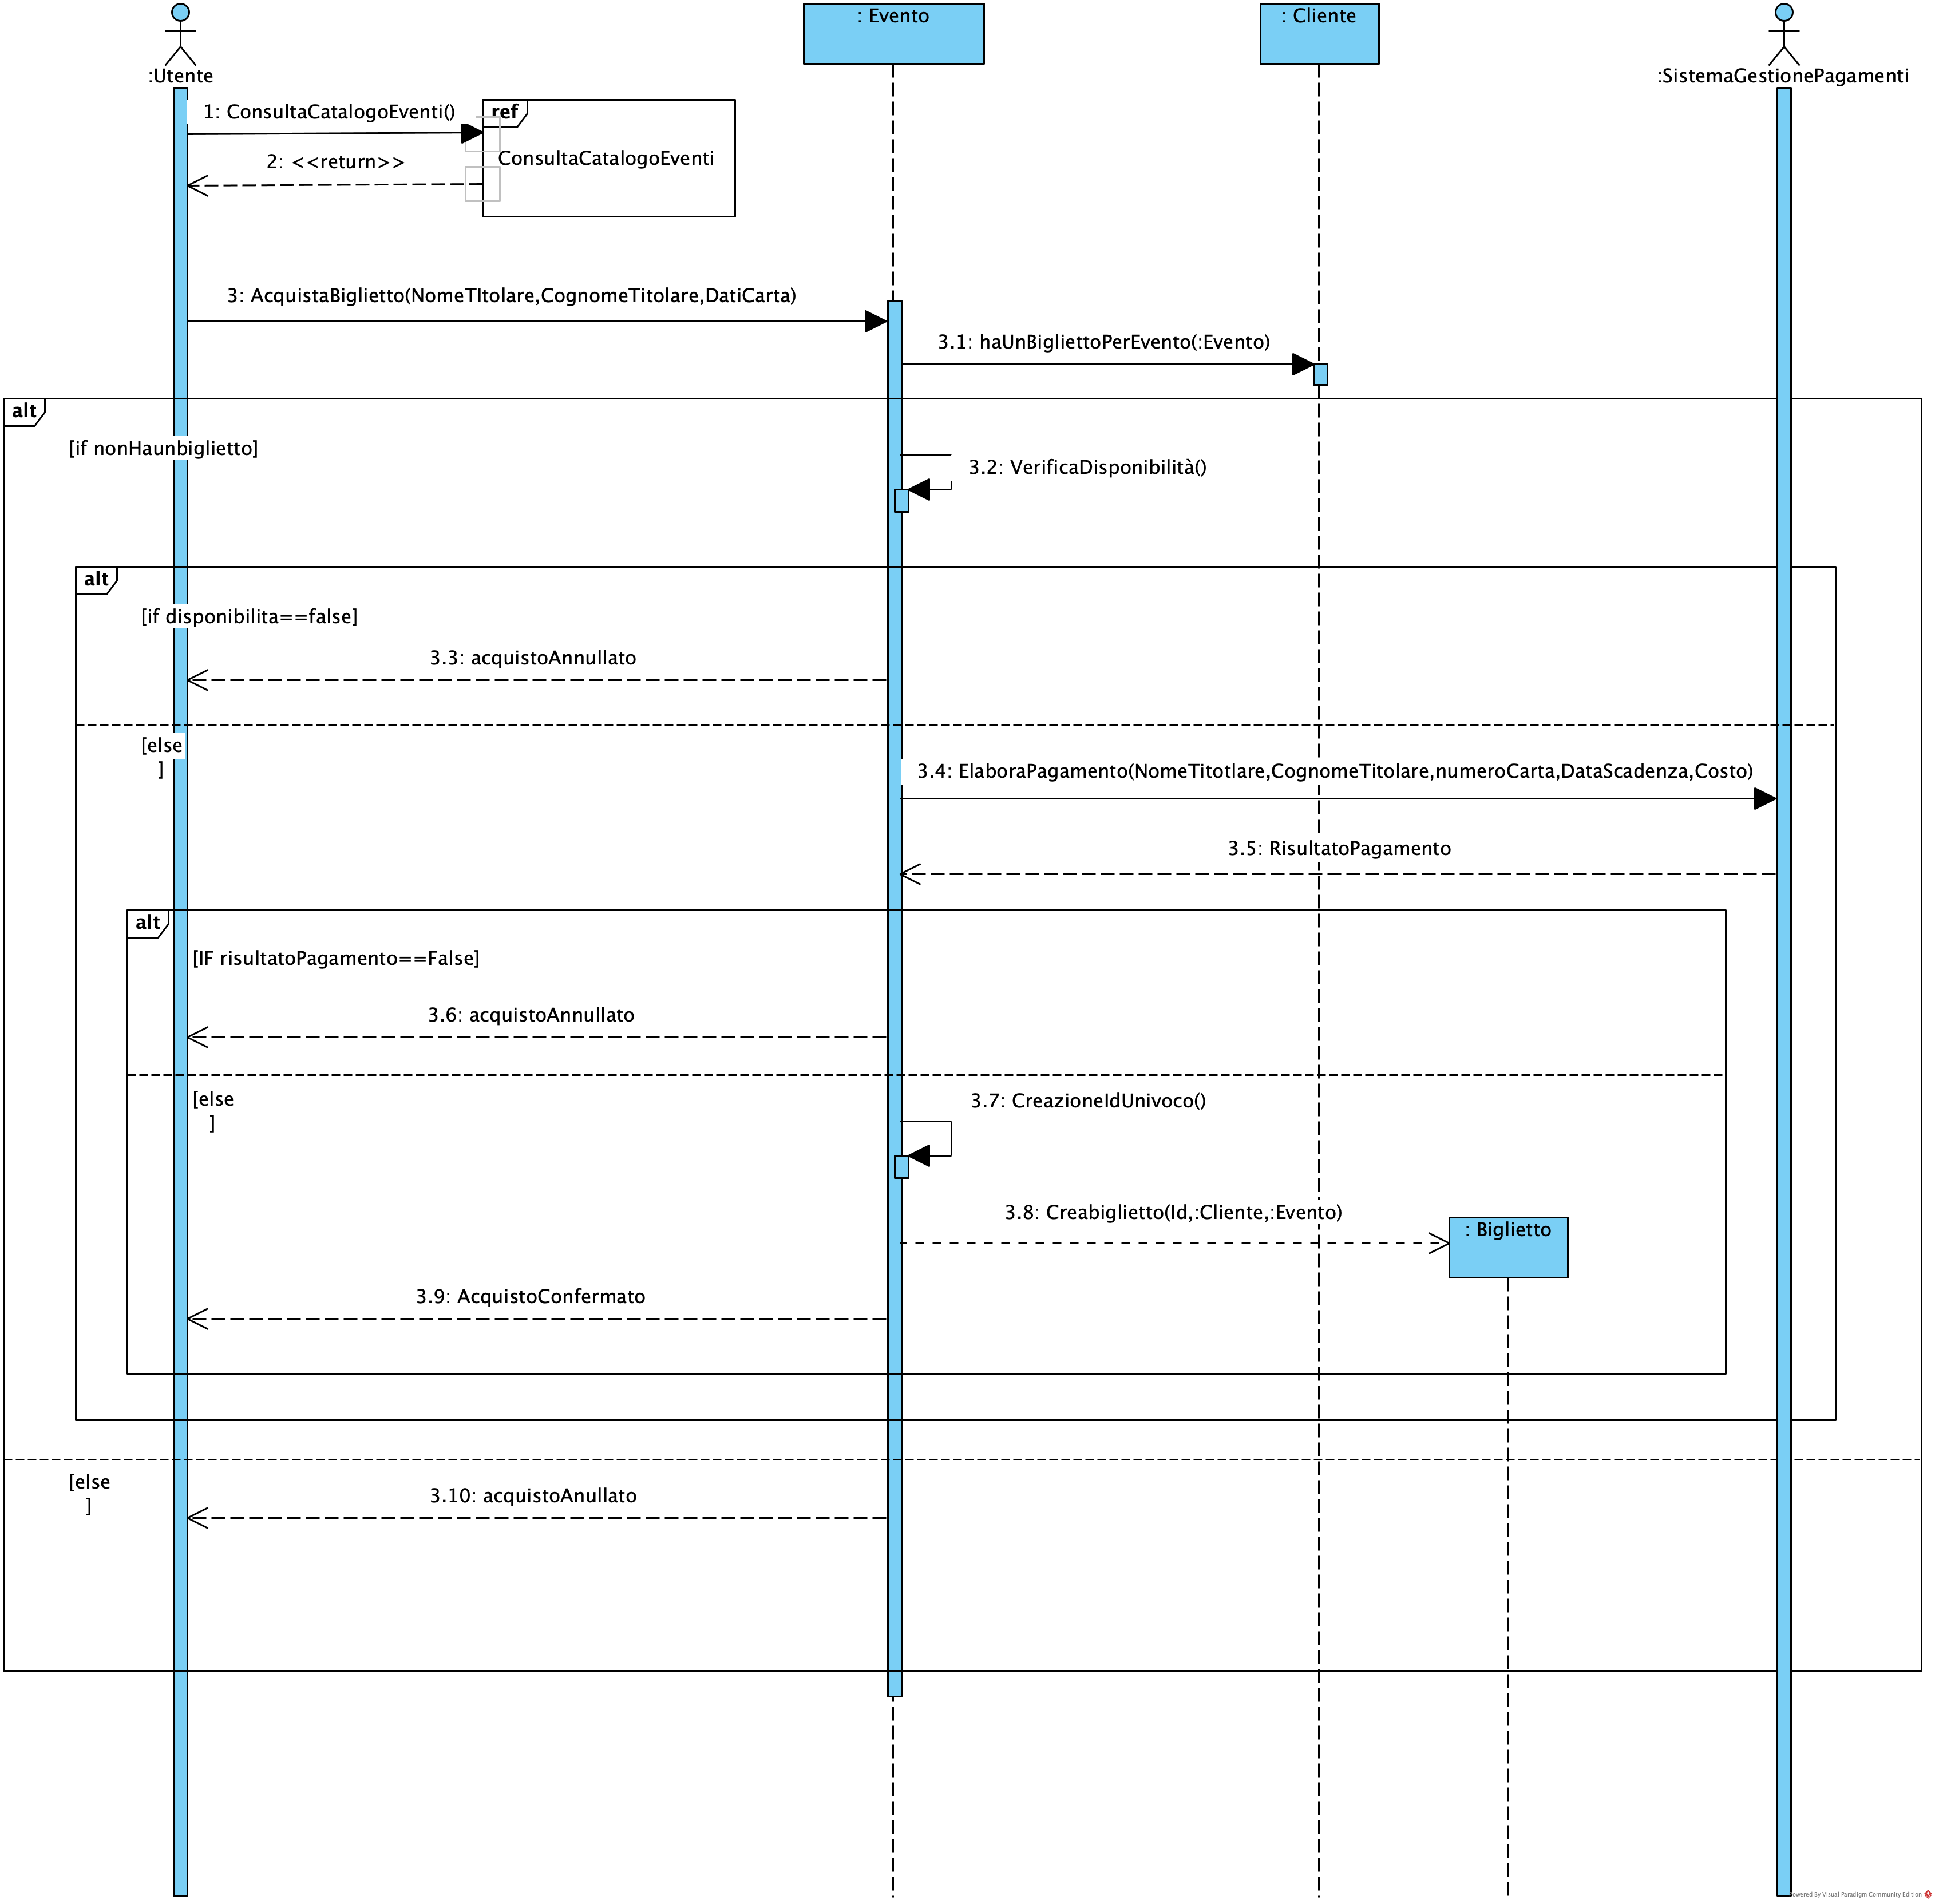
\includegraphics[width=0.8\linewidth]{assets/casid'uso/AcquistoBiglietto.png}
    \caption{Diagramma di sequenza per il caso d'uso \emph{AcquistoBiglietto}}
    \label{fig:acquistobiglietto}
\end{figure}


\newpage
\subsection{PartecipazioneEvento}

Il diagramma di sequenza ha evidenziato la necessità di aggiungere il metodo \texttt{verificaCodice()} per la classe \textbf{Evento}, il metodo \texttt{validaBiglietto()} per la classe \textbf{Biglietto} e il metodo \texttt{verificaBiglietto(Cliente)} per la classe \texttt{Biglietto}, necessari per gestire la partecipazione degli utenti agli eventi.

\begin{figure}[H]
    \centering
    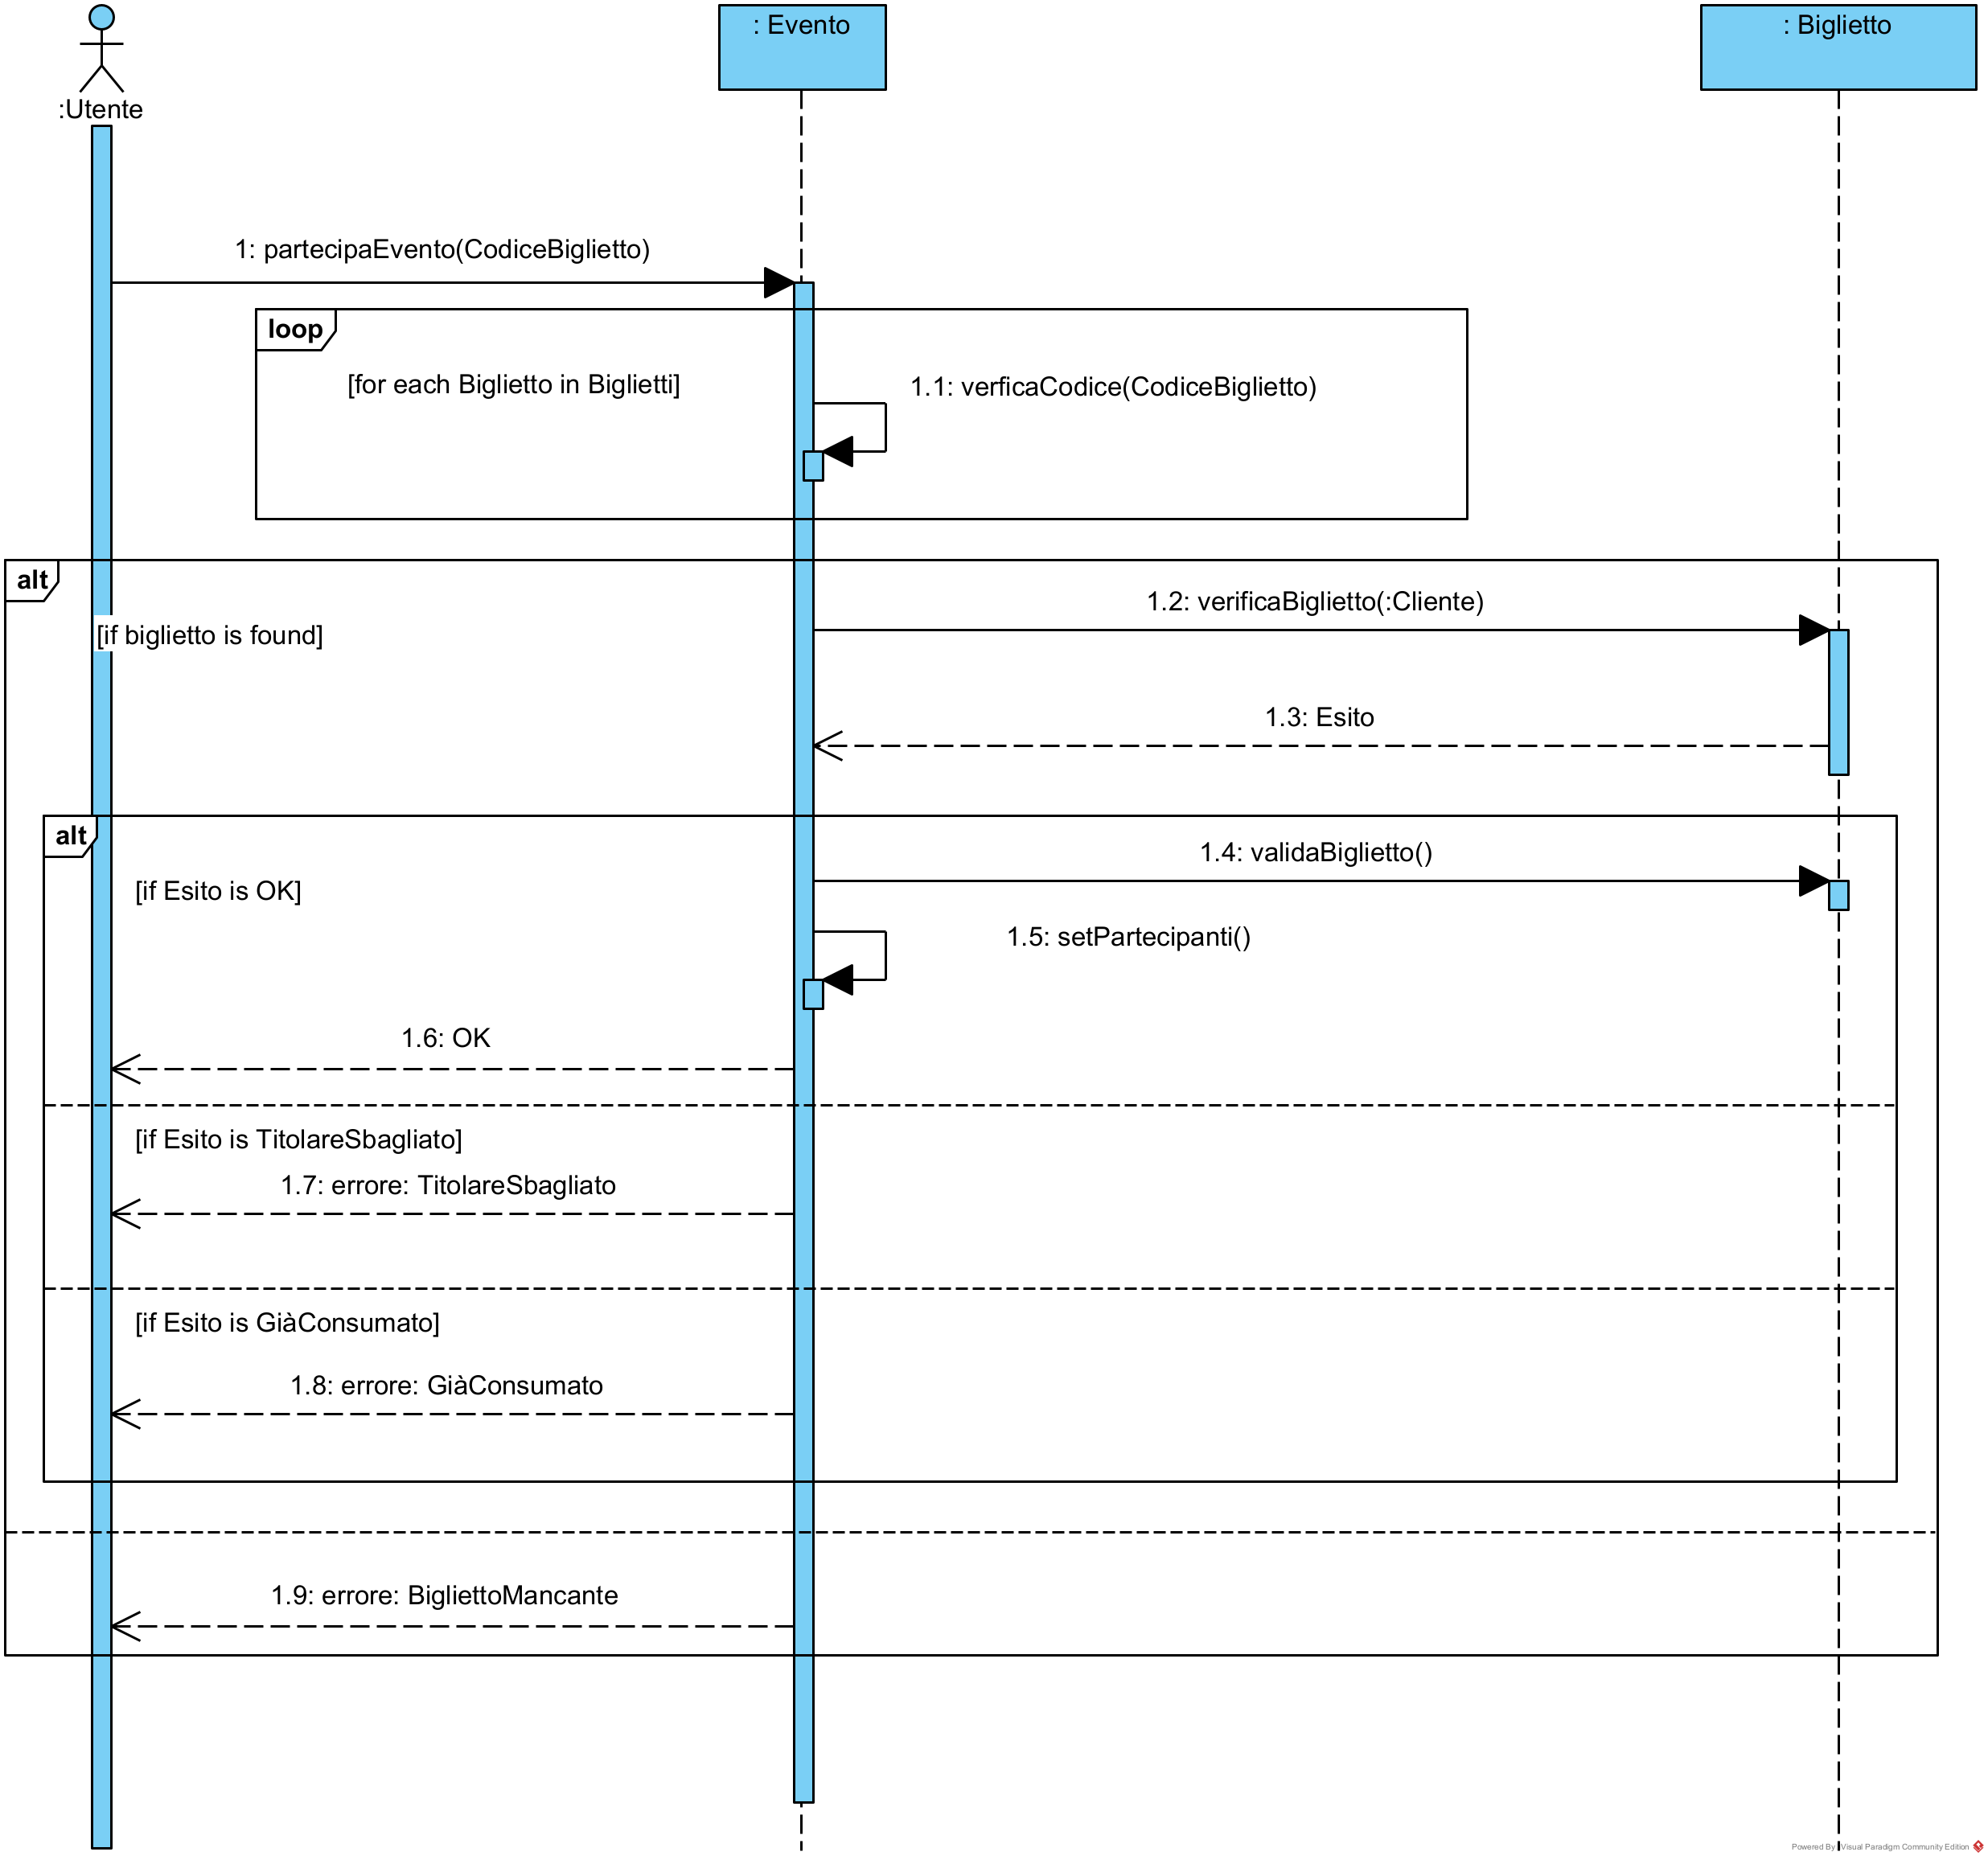
\includegraphics[height=0.38\textheight]{assets/casid'uso/PartecipazioneEvento.png}
    \caption{Diagramma di sequenza per il caso d'uso \emph{PartecipazioneEvento}}
    \label{fig:partecipazione}
\end{figure}

\section{Diagramma delle classi raffinato}
\begin{center}	
	\vspace{1ex}
	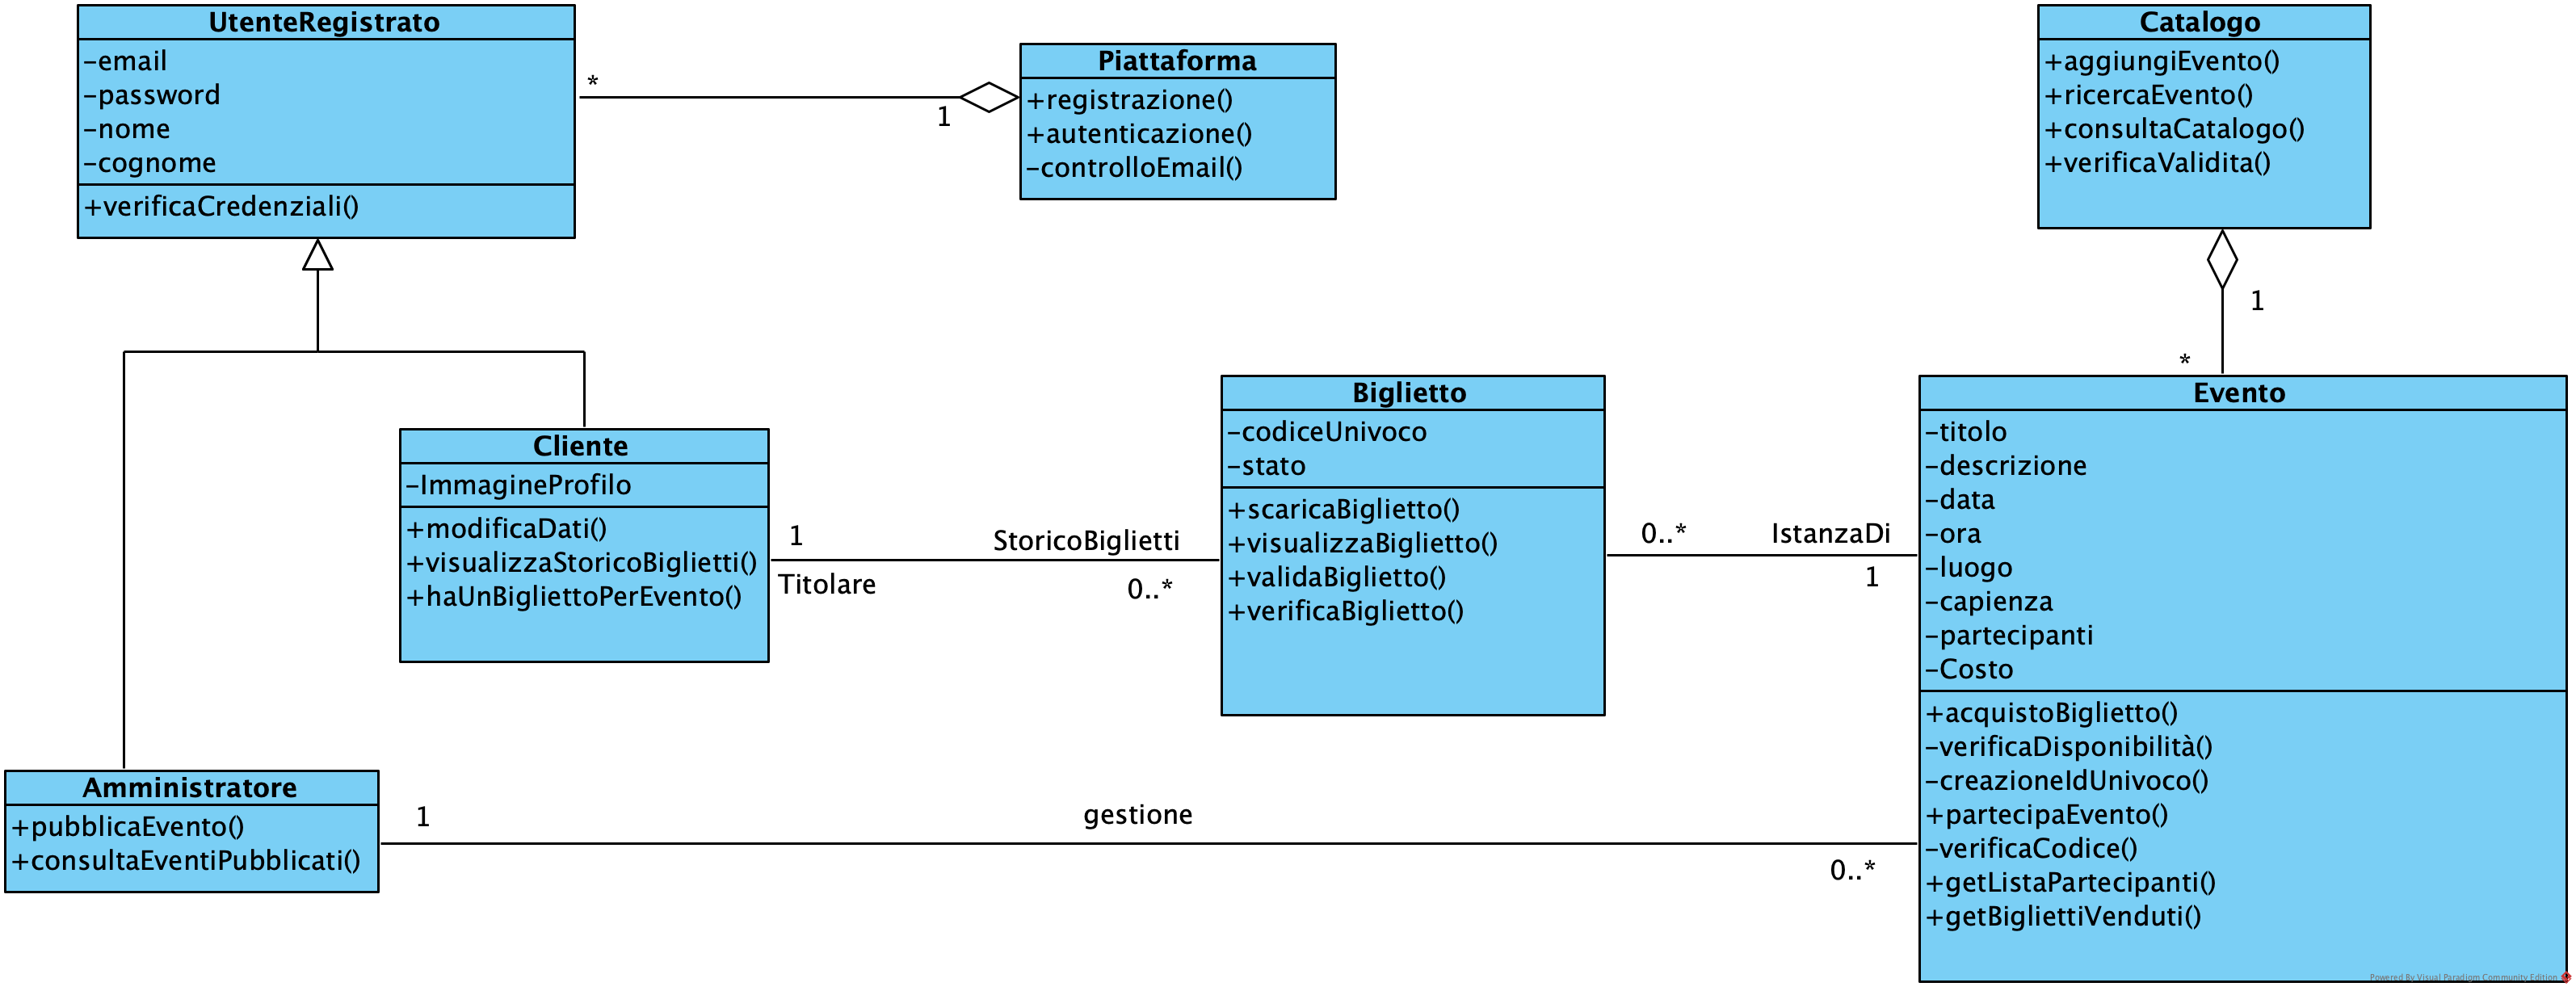
\includegraphics[height=0.38\linewidth]{assets/casid'uso/DiagrammaDelleClassiRaffinato.png}
	\vspace{1ex}
\end{center}